\documentclass{beamer}
\usetheme{Madrid}
\usecolortheme{beaver}
\usepackage{graphicx}
\graphicspath{{pics}}
\usepackage{listings}
\usepackage{xcolor}
\usepackage{tikz}
\usepackage{tcolorbox}
% Define custom colors
\definecolor{background}{RGB}{240,240,240}  % Light gray
\definecolor{keyword}{RGB}{0,102,204}       % Blue
\definecolor{comment}{RGB}{0,153,51}        % Green
\definecolor{string}{RGB}{204,51,0}         % Dark red
\definecolor{identifier}{RGB}{0,0,0}        % Black
\definecolor{number}{RGB}{153,0,153}        % Purple

\lstdefinestyle{colorful}{
    backgroundcolor=\color{background},
    keywordstyle=\color{keyword}\bfseries,
    commentstyle=\color{comment}\itshape,
    stringstyle=\color{string},
    identifierstyle=\color{identifier},
    numberstyle=\color{number},
    basicstyle=\ttfamily\small,
    breaklines=true,
    frame=single,
    framerule=2pt,
    rulecolor=\color{keyword},
    numbersep=8pt,
    numberstyle=\color{number},
    showstringspaces=false,
    tabsize=4,
    language=Python
}
\title{Introduction to Python, Data Structures and Algorithms}
\author{Nithin Vadekkapat}
\date{\today}

\begin{document}

\begin{frame}
    \titlepage
\end{frame}

\begin{frame}
    \frametitle{Table of Contents}
    \tableofcontents
\end{frame}


\section{Introduction}
\begin{frame}{What is Computer Science?}
    \begin{itemize}
        \item Computer Science is not merely the study of computers.
        \item Computers are tools that aid in problem-solving.
        \item The focus is on problems, problem-solving, and algorithmic solutions.
    \end{itemize}
\end{frame}

\begin{frame}{The Role of Algorithms}
    \begin{itemize}
        \item An algorithm is a step-by-step set of instructions to solve a problem.
        \item Some problems may not have a solution.
        \item Computer Science studies both solvable and unsolvable problems.
    \end{itemize}
\end{frame}

\begin{frame}{Computability in Computer Science}
    \begin{itemize}
        \item A problem is \textbf{computable} if an algorithm exists to solve it.
        \item Computer Science studies both computable and non-computable problems.
        \item Solutions are independent of the machine used.
    \end{itemize}
\end{frame}

\begin{frame}{Abstraction in Computer Science}
    \begin{itemize}
        \item Abstraction helps separate the logical and physical perspectives.
        \item Example: Driving a car.
        \item Users interact with the interface without needing to understand the mechanics.
    \end{itemize}
\end{frame}

\begin{frame}[fragile]{Procedural Abstraction}
    \begin{itemize}
        \item Users (clients) do not need to know implementation details.
        \item The interface provides a way to interact with complex implementations.
        \item Example: Python's \texttt{math} module.
    \end{itemize}

    \vspace{0.5cm} % Adds space for better readability

    
    \begin{lstlisting}[style=colorful, language=Python]
import math
math.sqrt(16)
    \end{lstlisting}

    \vspace{0.5cm} % Adds space before continuing the list

    \begin{itemize}
        \item We do not need to know how \texttt{sqrt} is implemented.
        \item We only need to know its name and how to use it.
    \end{itemize}
\end{frame}

\begin{frame}{Programming and Algorithms}
    \begin{itemize}
        \item Programming is encoding an algorithm into a notation (programming language) for computer execution
        \item Without an algorithm, there can be no program
        \item Computer science is not just programming, but programming is an essential part
        \item Programming creates representations of our solutions
    \end{itemize}
\end{frame}

\begin{frame}{From Algorithms to Programs}
    \begin{itemize}
        \item Algorithms describe solutions in terms of:
        \begin{itemize}
            \item Data needed to represent the problem instance
            \item Steps necessary to produce the intended result
        \end{itemize}
        \item Programming languages must provide notation for both process and data
        \item Languages provide control constructs and data types
    \end{itemize}
\end{frame}

\begin{frame}{Control Constructs}
    \begin{itemize}
        \item Control constructs allow algorithmic steps to be represented unambiguously
        \item Minimum requirements for algorithm representation:
        \begin{itemize}
            \item Sequential processing
            \item Selection for decision-making
            \item Iteration for repetitive control
        \end{itemize}
        \item Any language with these basic statements can represent algorithms
    \end{itemize}
\end{frame}

\begin{frame}{Data Types}
    \begin{itemize}
        \item All data in computers are strings of binary digits
        \item Data types provide interpretation for binary data
        \item Built-in/primitive data types are building blocks for algorithm development
        \item Example: Integer data type
        \begin{itemize}
            \item Binary digits interpreted as familiar numbers (23, 654, -19)
            \item Supports operations like addition, subtraction, multiplication
        \end{itemize}
    \end{itemize}
\end{frame}

\begin{frame}{Complexity Challenges}
    \begin{itemize}
        \item Problems and solutions are often very complex
        \item Simple language-provided constructs and data types:
        \begin{itemize}
            \item Are sufficient to represent complex solutions
            \item But can be at a disadvantage during problem-solving
        \end{itemize}
        \item Higher-level abstractions help manage this complexity
    \end{itemize}
\end{frame}

\begin{frame}{Abstraction in Problem-Solving}
    \begin{itemize}
        \item Computer scientists use abstractions to focus on the ``big picture''
        \item Creating models of the problem domain enables:
        \begin{itemize}
            \item More efficient problem-solving process
            \item More consistent description of data with respect to the problem
        \end{itemize}
        \item Abstractions allow us to ignore implementation details temporarily
    \end{itemize}
\end{frame}

\begin{frame}{Data Abstraction}
    \begin{itemize}
        \item Abstract Data Type (ADT): logical description of data and operations
        \item Focuses on \textit{what} the data represents, not \textit{how} it's constructed
        \item Creates encapsulation around data through information hiding
        \item Users interact with the interface only, not the implementation
    \end{itemize}
\end{frame}

\begin{frame}{ADT Implementation}
    \begin{itemize}
        \item Implementation of an ADT is called a data structure
        \item Data structure provides the physical view of the data
        \item Uses programming constructs and primitive data types
        \item Different implementations can satisfy the same ADT
        \item Choice of implementation affects efficiency
    \end{itemize}
\end{frame}


\section{Atomic Data Types}
\begin{frame}{Objects}
    \begin{itemize}
        \item Everything in Python is an object
        \item Objects have attributes and methods
        \item Objects can be created from classes
        \item Classes define the attributes and methods of objects
    \end{itemize}
\end{frame}
\begin{frame}
    \begin{figure}
        \centering
        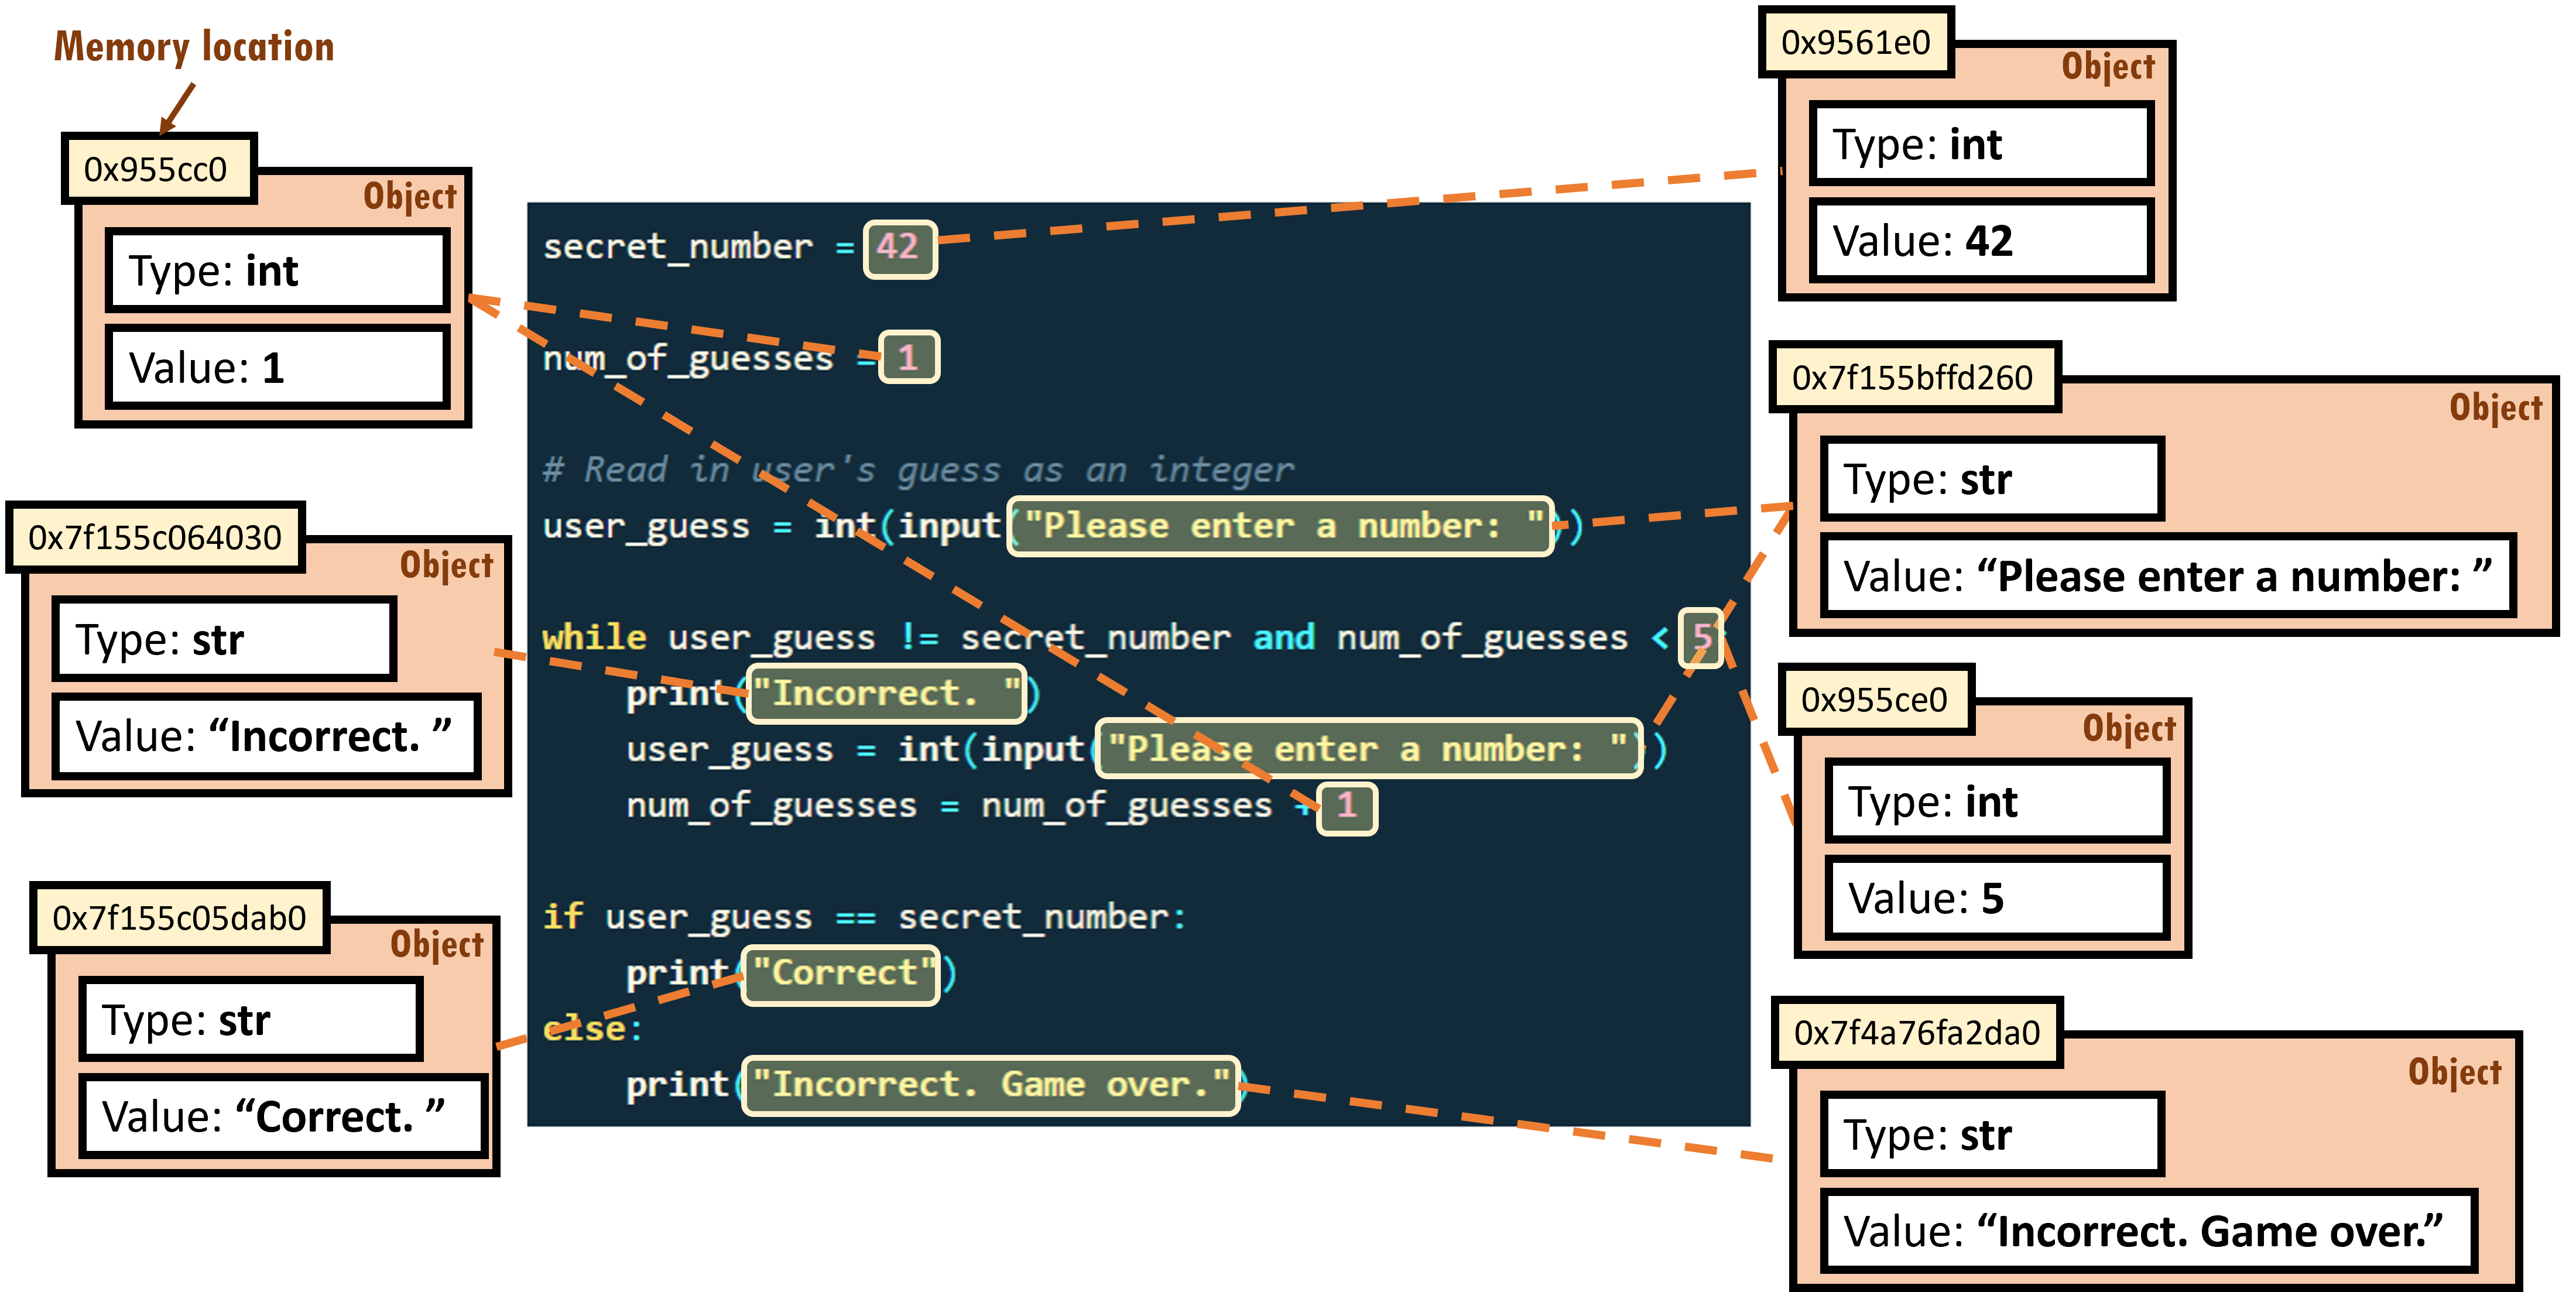
\includegraphics[width=1.0\textwidth]{pics/objects.png}
        \caption{Objects in Python}
    \end{figure}
\end{frame}
\begin{frame}{Built in atomic datatypes}
    \begin{itemize}
        \item Python provides built-in data types
        \item These types are used to represent data in programs
        \item Common data types include:
        \begin{itemize}
            \item Integers
            \item Floats
            \item Strings
            \item Booleans
        \end{itemize}
    \end{itemize}
\end{frame}
\begin{frame}{Operators and Expressions}
    \begin{columns}
        \column{0.5\textwidth}
        \begin{itemize}
            \item Objects can be combined using operators
            \item Arithmrtic operators in python 
            \begin{itemize}
            \item \texttt{+} (addition)
            \item \texttt{-} (subtraction)
            \item \texttt{*} (multiplication)
            \item \texttt{/} (division)
            \item \texttt{//} (floor division, or integer part of division)
            \item \texttt{\%} (modulo, or remainder after division)
            \item \texttt{**} (exponential -- raised to the power)
            \end{itemize}
                    \end{itemize}
        \column{0.5\textwidth}
        \begin{figure}
            \centering
            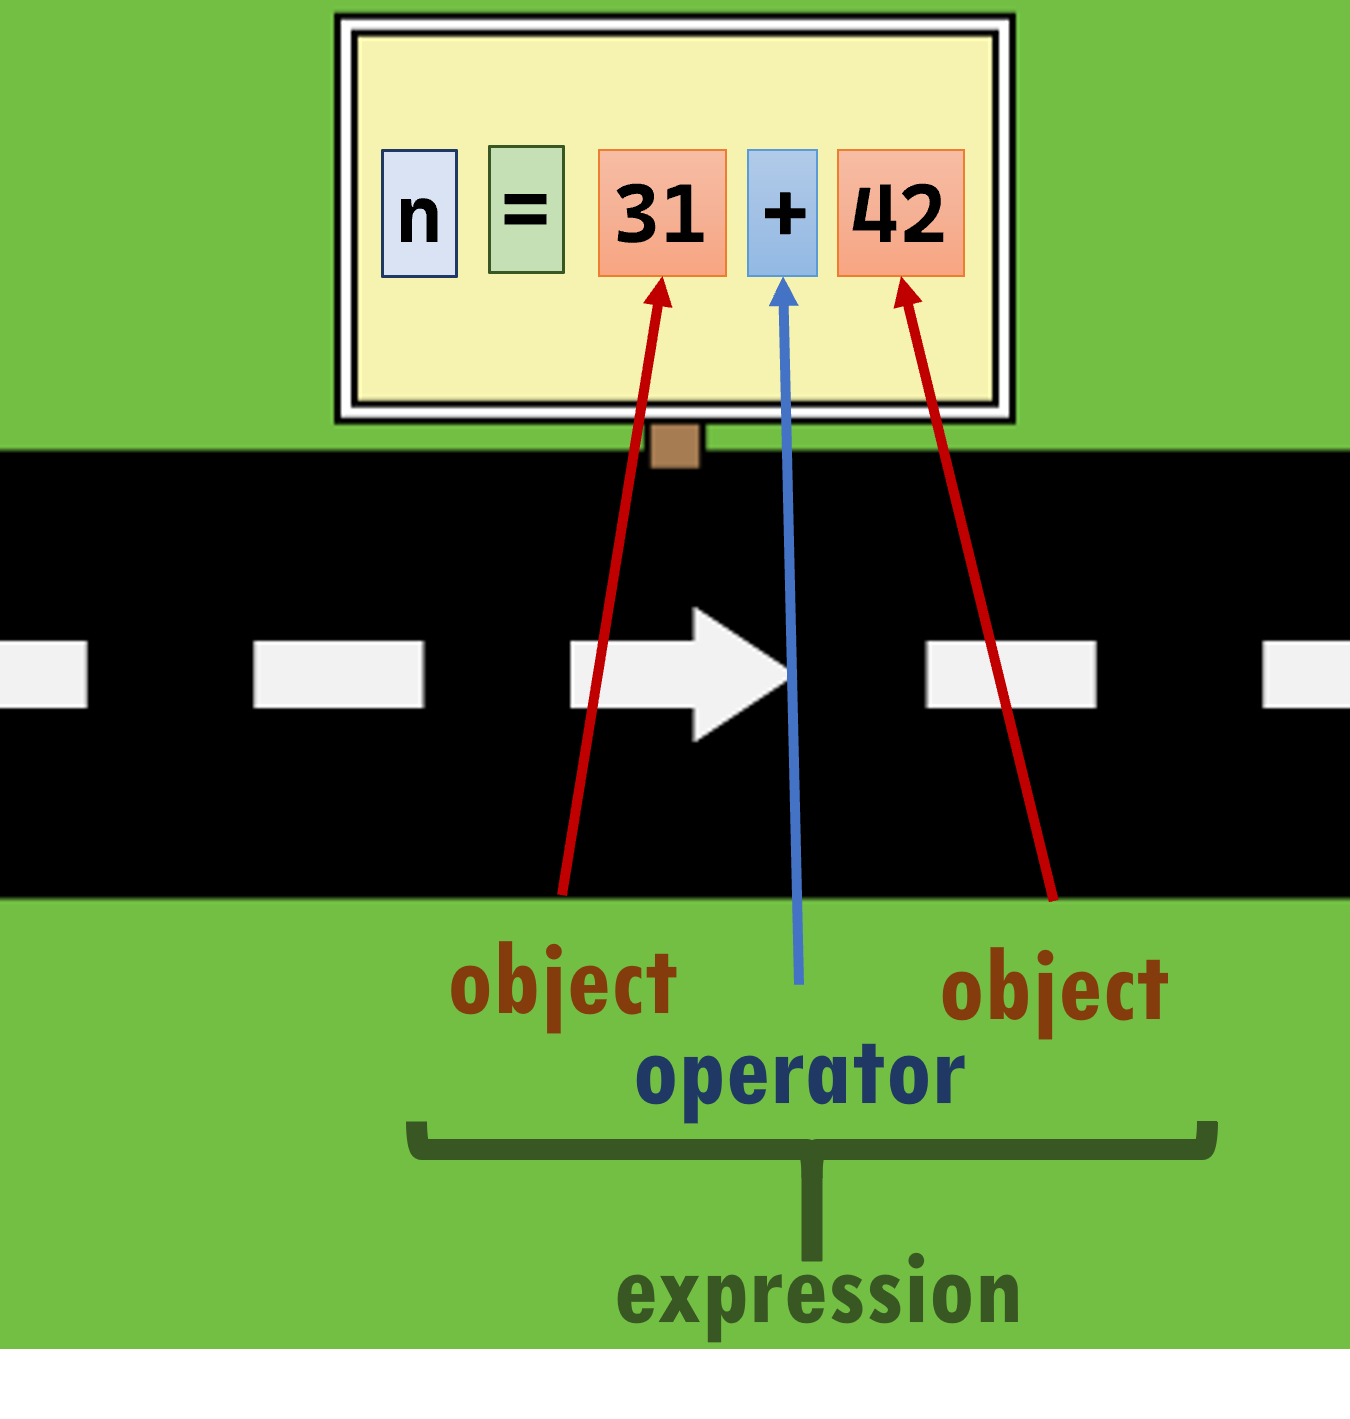
\includegraphics[width=0.8\textwidth]{pics/operator.png}
            \caption{Operators in Python}
        \end{figure}
    \end{columns}
\end{frame}
\begin{frame}{Python Operator Precedence}
    \begin{itemize}
        \item Python evaluates expressions based on operator precedence.
        \item Common operators in order of precedence (from highest to lowest):
        \begin{itemize}
            \item \texttt{()} -- Parentheses
            \item \texttt{**} -- Exponentiation
            \item \texttt{+x}, \texttt{-x}, \texttt{\textasciitilde{}x} -- Unary plus, Unary minus, Bitwise NOT
            \item \texttt{*}, \texttt{/}, \texttt{//}, \texttt{\%} -- Multiplication, Division, Floor division, Modulus
            \item \texttt{+}, \texttt{-} -- Addition, Subtraction
            \item \texttt{<<}, \texttt{>>} -- Bitwise shift operators
            \item \texttt{\&} -- Bitwise AND
            \item \texttt{\textasciicircum} -- Bitwise XOR
            \item \texttt{|} -- Bitwise OR
            \item \texttt{==}, \texttt{!=}, \texttt{>}, \texttt{<}, \texttt{>=}, \texttt{<=}, \texttt{is}, \texttt{is not}, \texttt{in}, \texttt{not in} -- Comparisons, Identity, Membership
            \item \texttt{not} -- Logical NOT
            \item \texttt{and} -- Logical AND
            \item \texttt{or} -- Logical OR
        \end{itemize}
        \item Example: \texttt{1 + 2 * 3 == 7} evaluates as \texttt{1 + (2 * 3) == 7}, which is \texttt{1 + 6 == 7}, resulting in \texttt{True}.
    \end{itemize}
\end{frame}
\begin{frame}[fragile]{Overloaded Operators}
    \begin{itemize}
        \item Some operators are not limited to arithmetic operations with numbers.
        \item For example, \texttt{+} and \texttt{*} can be used for a different kind of operation when used with strings.
    \end{itemize}
    \begin{lstlisting}[style=colorful, language=Python]
>>> 'hello' + 'world'
'helloworld'
>>> 'hello' * 3
'hellohellohello'
    \end{lstlisting}
\end{frame}

\begin{frame}{Variables}
    In Python, a variable is simply a name or a label that points to an object instance in memory
    \begin{figure}
        \centering
        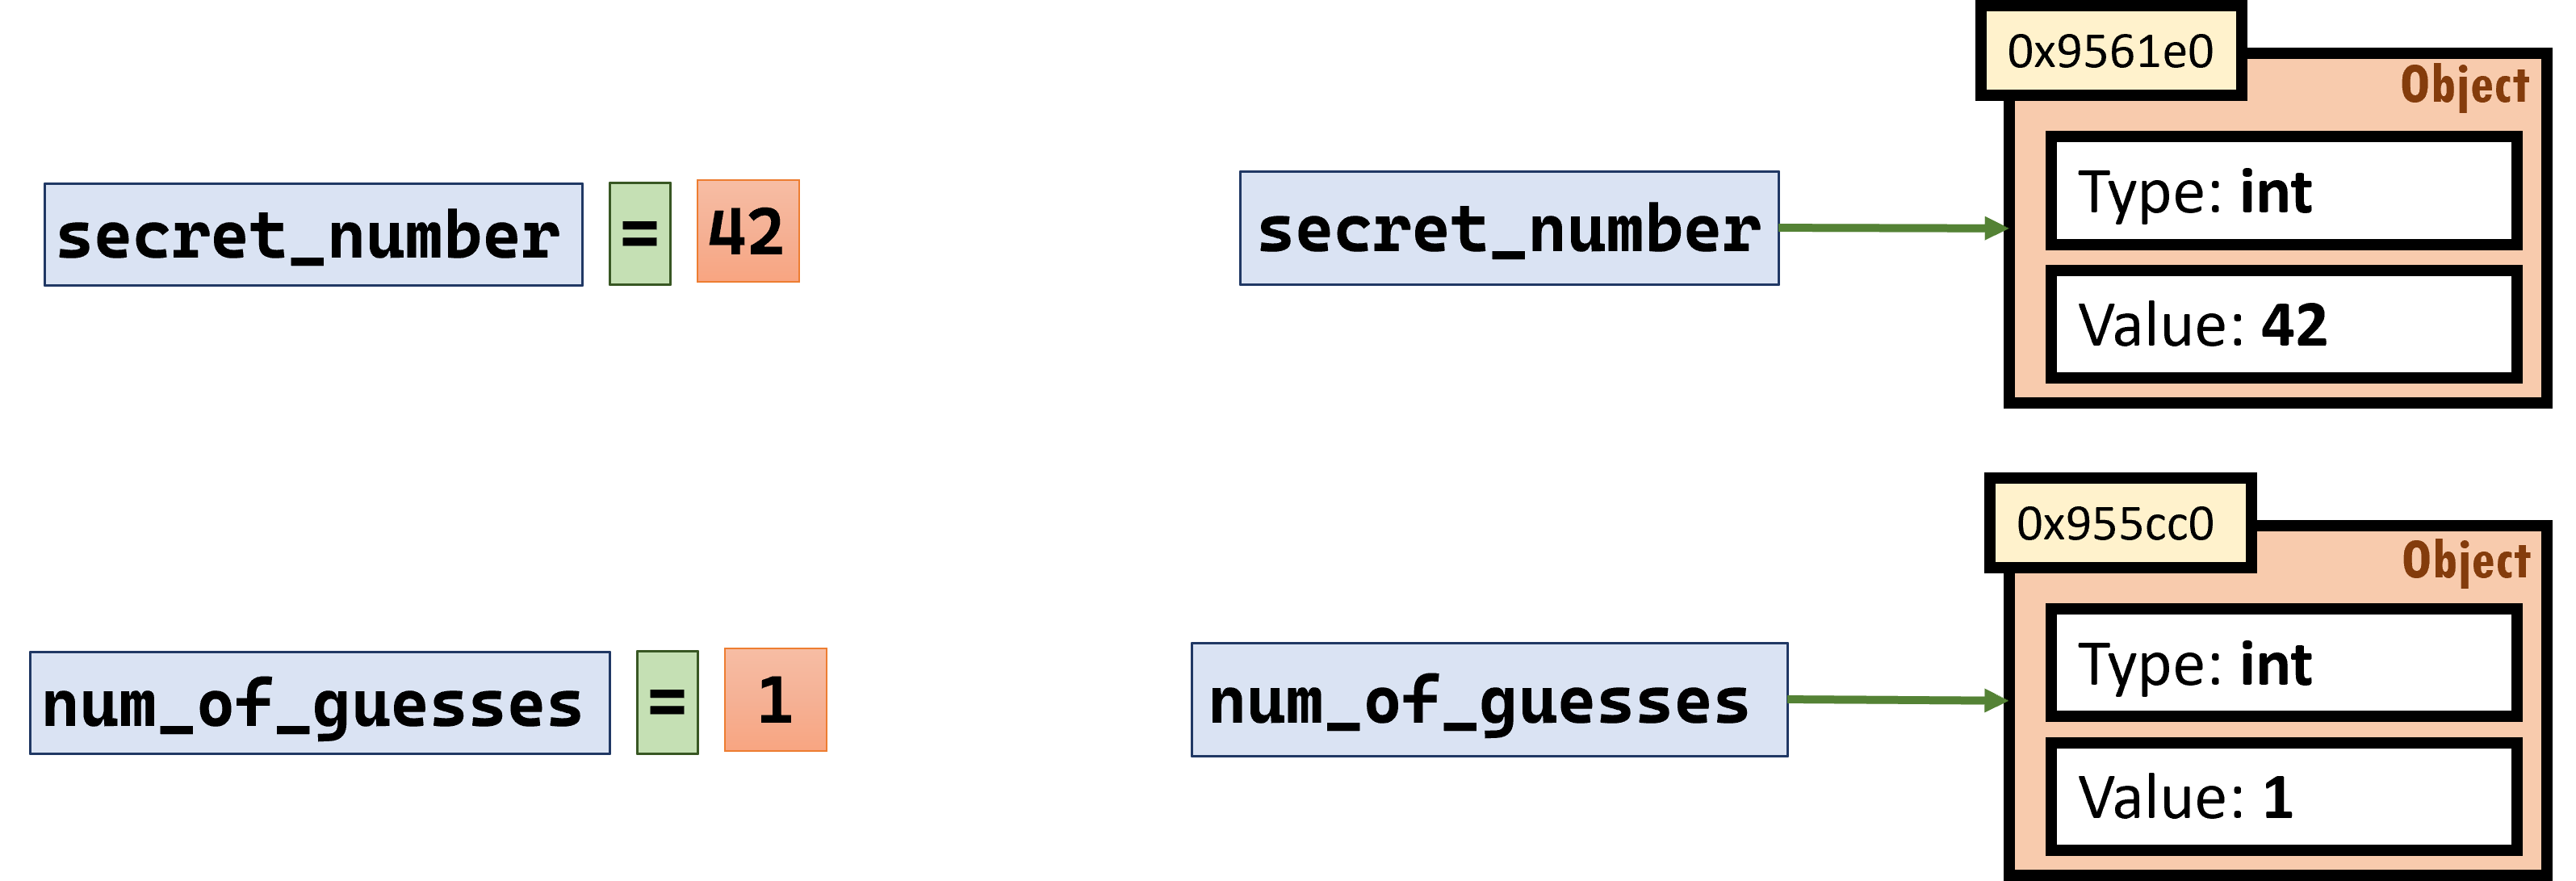
\includegraphics[width=0.8\textwidth]{pics/variable.png}
        \caption{Variables in Python}
    \end{figure}
\end{frame}

\begin{frame}{Variable Assignments}
    \begin{columns}
        \column{0.5\textwidth}
        \begin{figure}
            \centering
            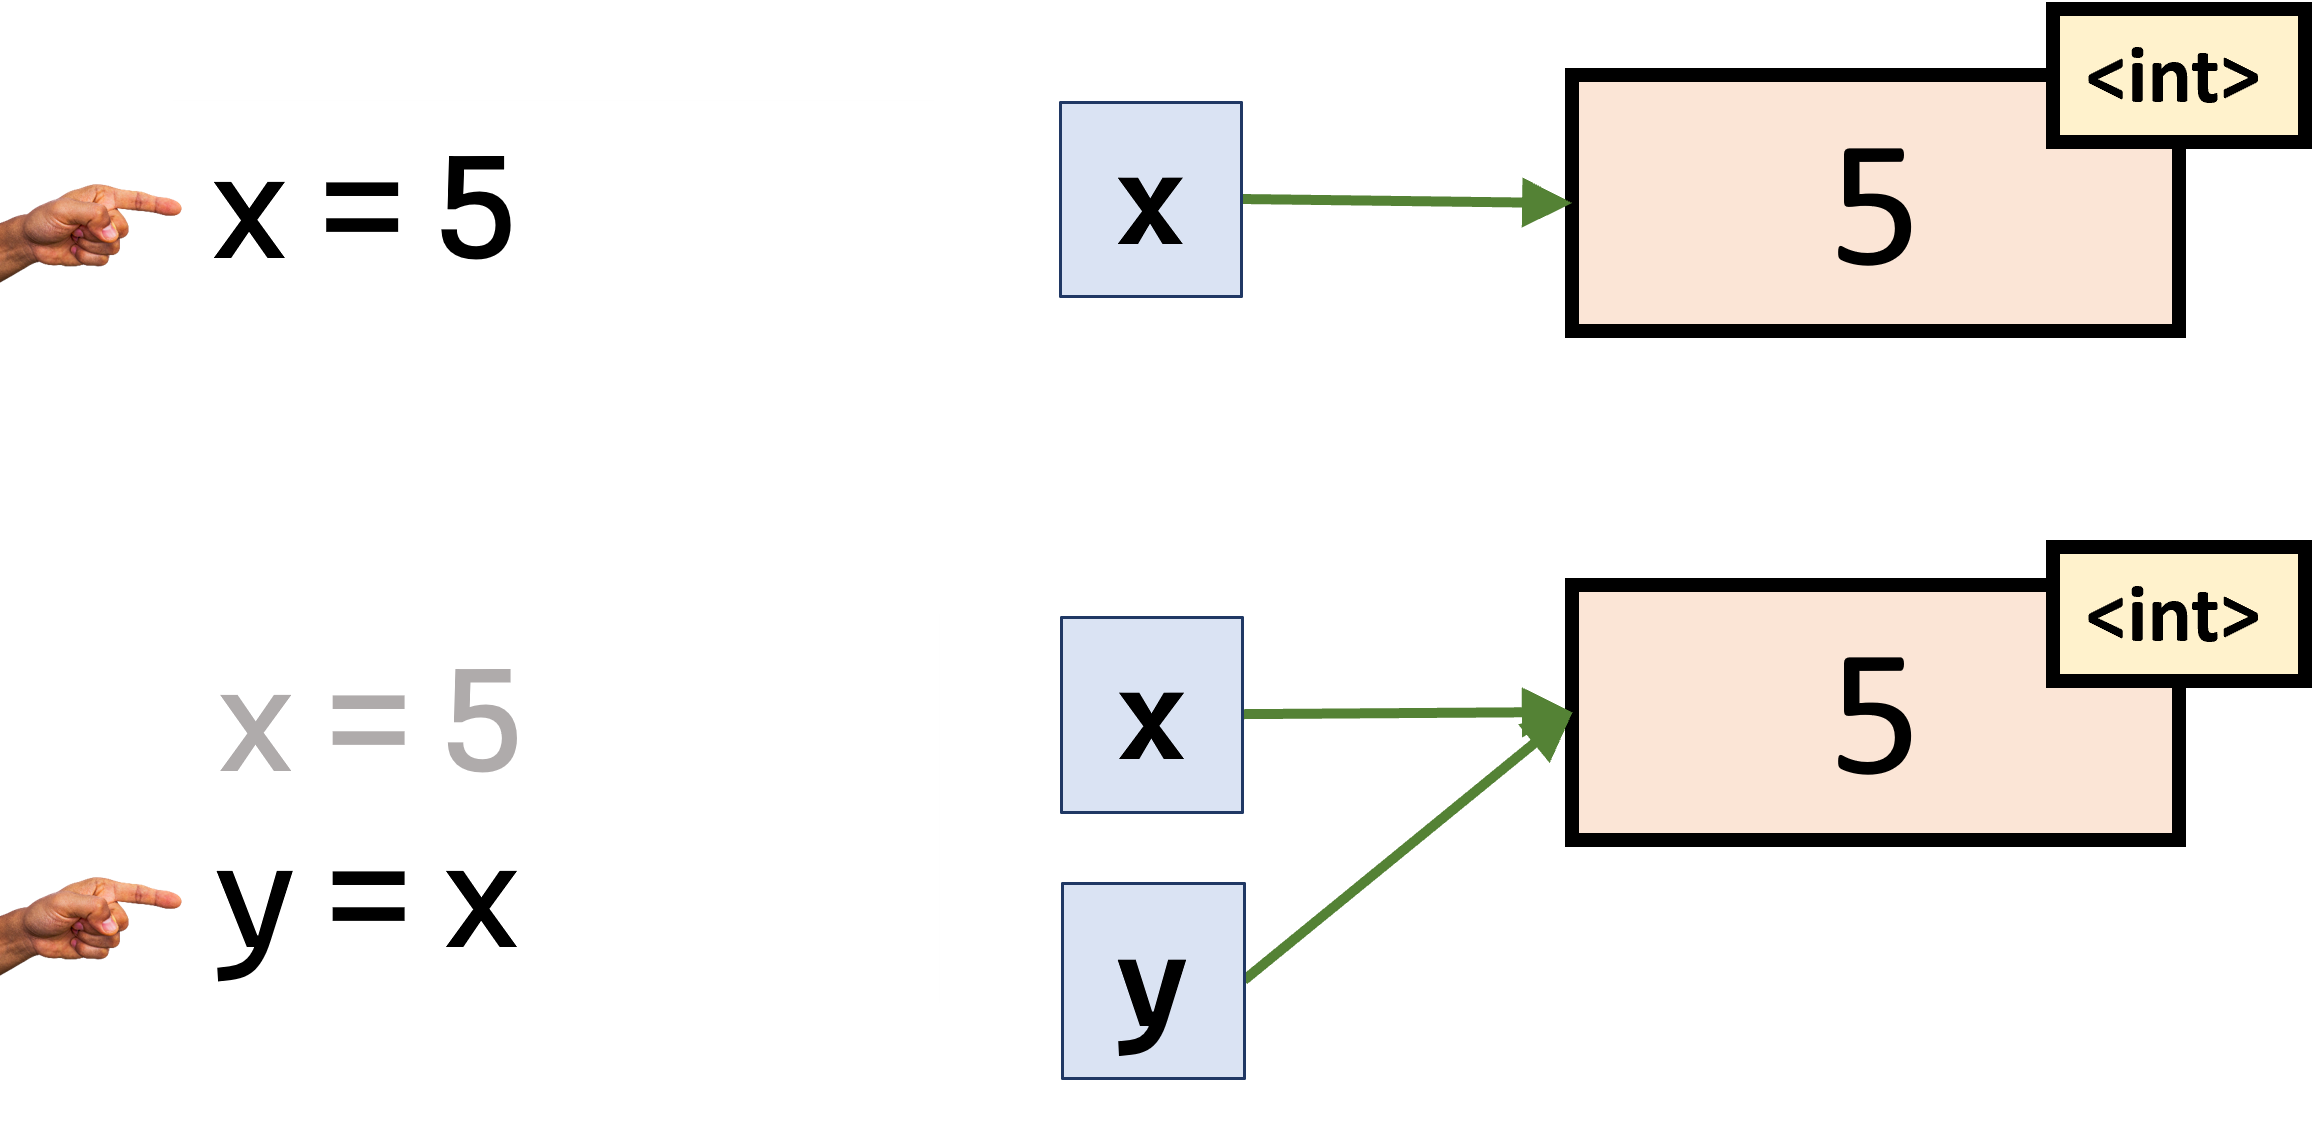
\includegraphics[width=0.8\textwidth]{pics/assignment.png}
            \caption{Variable Assignment}
        \end{figure}
        \column{0.5\textwidth}
        \begin{figure}
            \centering
            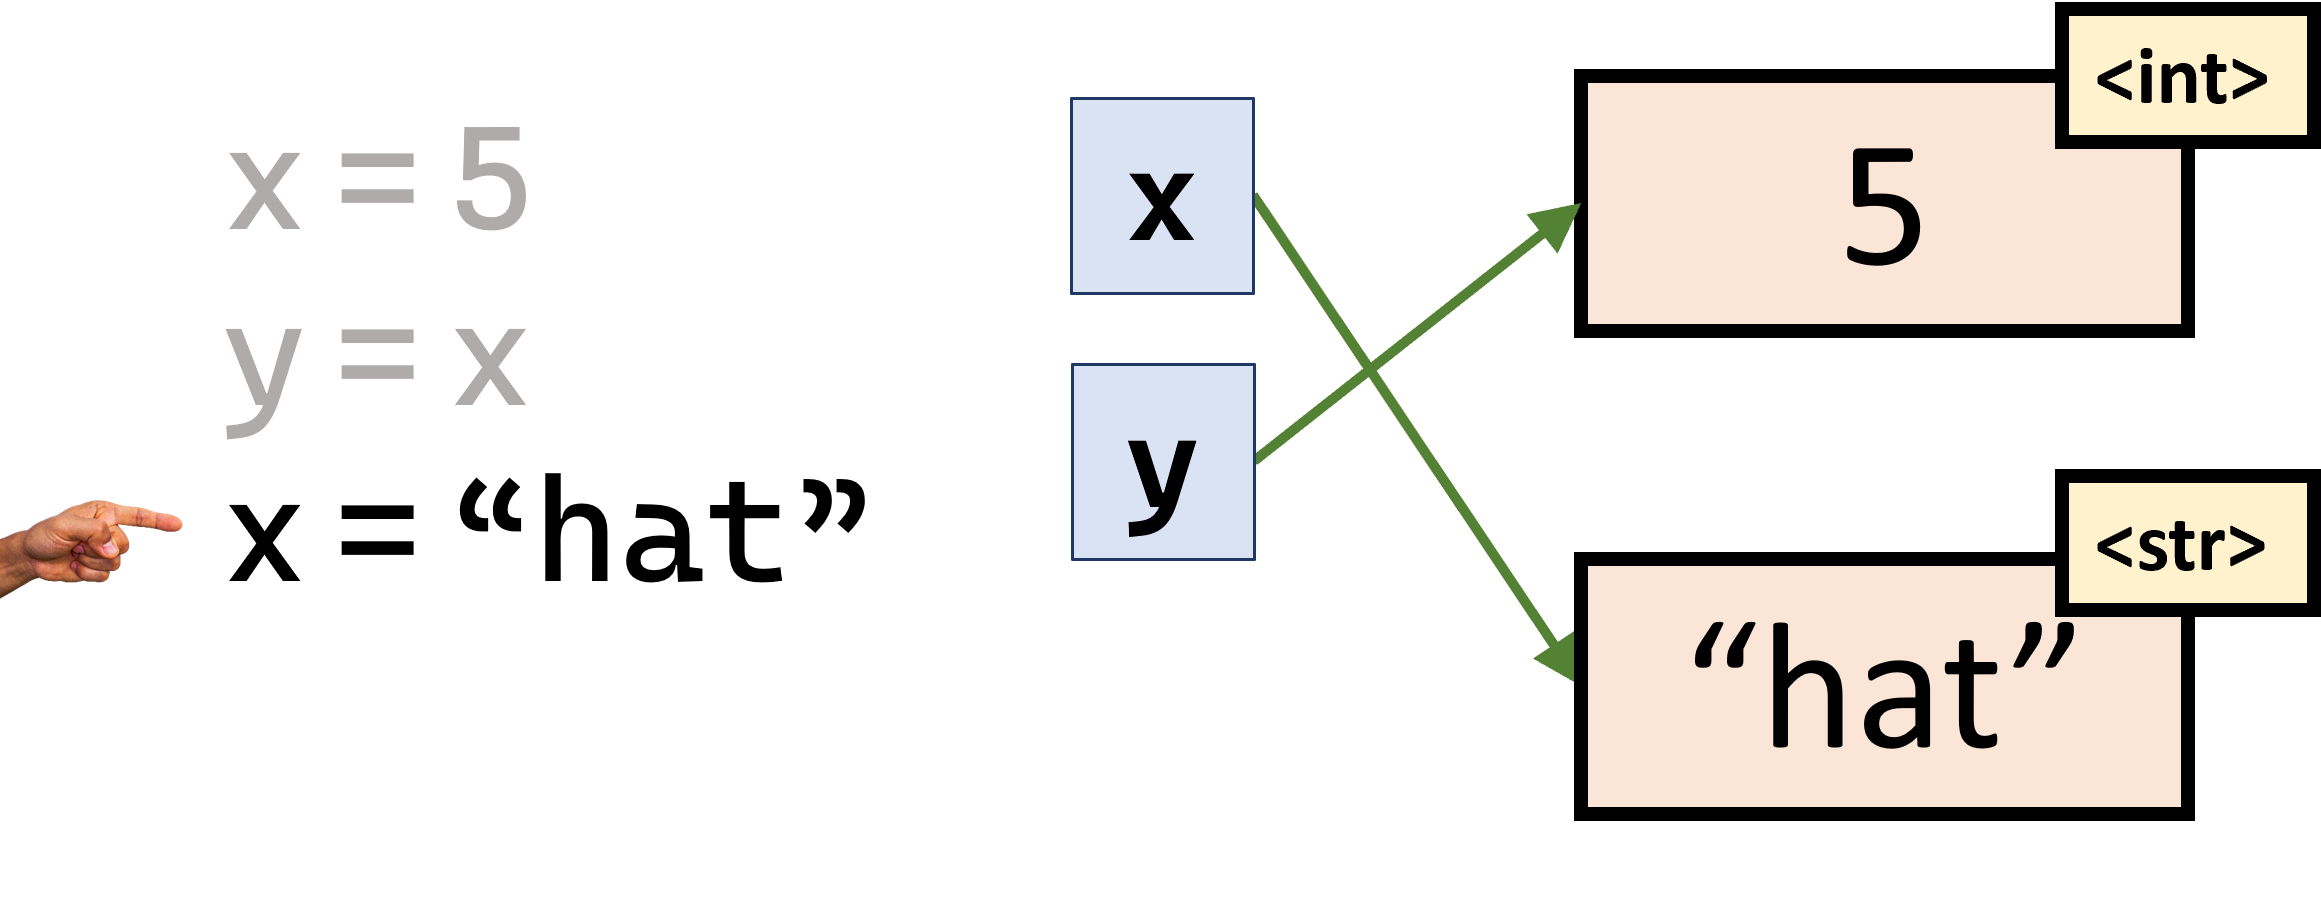
\includegraphics[width=0.8\textwidth]{pics/assignment2.png}
            \caption{Variable Assignment}
        \end{figure}
    \end{columns}
    
\end{frame}

\begin{frame}[fragile]{Variable Assignment}
    \begin{lstlisting}[style=colorful, language=Python]
>>> x = 20
>>> y = x
>>> x = "hello"
>>> print(y)
20
>>> print(x)
hello
    \end{lstlisting}
\end{frame}


\begin{frame}{Naming Variables}
    \begin{itemize}
        \item Variable names must start with a letter or an underscore
        \item The rest of the name can contain letters, numbers, and underscores
        \item Variable names are case-sensitive
        \item Variable names should be descriptive
    \end{itemize}
\end{frame}

\begin{frame}[fragile]{Reserved Keywords}
    \begin{lstlisting}[style=colorful, language=Python]
     >>> import keyword
     >>> keyword.kwlist      
    \end{lstlisting}
\end{frame} 

\begin{frame}
    \frametitle{Comparison Operators}
    \begin{itemize}
        \item Comparison operators are used to compare two values
        \item They return a boolean value (True or False)
        \item Common comparison operators include:
        \begin{itemize}
            \item \texttt{==} (equal to)
            \item \texttt{!=} (not equal to)
            \item \texttt{>} (greater than)
            \item \texttt{<} (less than)
            \item \texttt{>=} (greater than or equal to)
            \item \texttt{<=} (less than or equal to)
        \end{itemize}
    \end{itemize}
\end{frame}


\begin{frame}[fragile]{Python Quiz-1}
\begin{lstlisting}[style=colorful, language=Python]
>>> 5 == 5.0000
>>> 1+2 == 3 
>>> 9 > 8.999999999999999
>>> 6 // 3 == 6.0 / 3.0
\end{lstlisting}
\end{frame}

\begin{frame}[fragile]{Floating-Point Comparisons}
    \begin{itemize}
        \item Floating-point numbers can have precision issues due to their representation in memory.
        \item Comparisons involving equality can be affected by these precision issues.
        \item Example: \texttt{1.1 + 2.2 == 3.3} evaluates to \texttt{False} due to tiny inaccuracies.
        \item However, comparisons involving inequality are less likely to be affected.
        \item Example: \texttt{9 > 8.999999999999999} evaluates to \texttt{True}.
    \end{itemize}
    \begin{lstlisting}[style=colorful, language=Python]
>>> 1.1 + 2.2 == 3.3
False
>>> 9 > 8.999999999999999
True
    \end{lstlisting}
\end{frame}

\begin{frame}[fragile]
    \frametitle{Python Quiz-2}
    \begin{lstlisting}[style=colorful, language=Python]
>>> 5 != 5.0000
>>> True != False
>>> False < True
>>> "10" > "2"
    \end{lstlisting}
\end{frame}
\begin{frame}{What are Chained Comparisons?}
    \begin{itemize}
      \item Python allows multiple comparison operators to be chained together in a single expression.
      \item This creates a more readable and concise way to express complex comparisons.
      \item The comparisons are evaluated from left to right, and they are implicitly combined using the logical \texttt{and} operator.
    \end{itemize}
  \end{frame}
  
  \begin{frame}[fragile]{Example 1: Simple Range Check}
    \begin{itemize}
      \item Consider checking if a variable \texttt{x} is within a specific range.
      \item Without chained comparisons:
        \begin{lstlisting}[style=colorful, language=Python]
  if 10 < x and x < 20:
      # ...
        \end{lstlisting}
      \item With chained comparisons:
        \begin{lstlisting}[style=colorful, language=Python]
  if 10 < x < 20:
      # ...
        \end{lstlisting}
      \item Both are equivalent, but the chained version is more readable.
    \end{itemize}
  \end{frame}
  
  \begin{frame}[fragile]{Example 2: Multiple Comparisons}
    \begin{lstlisting}[style=colorful, language=Python]
  x = 5
  y = 10
  z = 15
  if x < y < z:
      print("x < y < z is True")
    \end{lstlisting}
    \begin{itemize}
      \item This checks if \texttt{x} is less than \texttt{y} AND \texttt{y} is less than \texttt{z}.
    \end{itemize}
  \end{frame}
  
  \begin{frame}[fragile]{Example 3: Equality and Inequality}
      \begin{lstlisting}[style=colorful, language=Python]
  a = 10
  b = 10
  c = 15
  if a == b < c:
      print("a==b<c is True")
      \end{lstlisting}
      \begin{itemize}
          \item This checks if \texttt{a} is equal to \texttt{b} AND \texttt{b} is less than \texttt{c}.
      \end{itemize}
  \end{frame}


\section{Collection Data Types}
\begin{frame}
    \frametitle{Builtin Collection Data Types}
    \begin{itemize}
        \item Python provides several collection data types
        \item These types are used to store multiple values in a single variable
        \item Common collection data types include:
        \begin{itemize}
            \item Lists
            \item Tuples
            \item Sets
            \item Dictionaries
        \end{itemize}
    \end{itemize}   
\end{frame}

\begin{frame}
    \frametitle{Lists}
    \begin{itemize}
        \item Lists are ordered collections of items
        \item Lists can contain items of different types
        \item Lists are mutable, meaning they can be changed after creation
        \item Lists are created using square brackets \texttt{[]}
    \end{itemize}
\end{frame}

\begin{frame}[fragile]{Creating Lists}
    \begin{lstlisting}[style=colorful, language=Python]
# Create an empty list
my_list = []
# Create a list with items
my_list = [1, 2, 3, 4, 5]  
my_another_list = ['a', 'b', 'c', False, 3, 0.11]  
    \end{lstlisting}
\end{frame}

\begin{frame}[fragile]{Accessing List Items}
    \begin{lstlisting}[style=colorful, language=Python]
# Access the first item in the list
print(my_list[0])
# Access the last item in the list
print(my_list[-1])
    \end{lstlisting}
\end{frame} 

\begin{frame}[fragile]{Slicing Lists}
    \begin{lstlisting}[style=colorful, language=Python]
# Get the first three items in the list
print(my_list[:3])
# Get the last three items in the list
print(my_list[-3:])
    \end{lstlisting}
\end{frame}             


\begin{frame}[fragile]{Adding Items to a List}
    \begin{lstlisting}[style=colorful, language=Python]
# Append an item to the end of the list
my_list.append(6)
# Insert an item at a specific index
my_list.insert(0, 0)
    \end{lstlisting}
\end{frame}     


\begin{frame}[fragile]{List Operations}
    \begin{lstlisting}[style=colorful, language=Python]
# Concatenate two lists
new_list = my_list + [7, 8, 9]
# Repeat a list
repeated_list = my_list * 2
    \end{lstlisting}
\end{frame}

\begin{frame}[fragile]{Mutability of Lists in Python}
    \begin{itemize}
        \item Lists in Python are mutable, meaning their contents can be changed after creation.
        \item Example: Modifying a list through a reference.
    \end{itemize}
    \begin{lstlisting}[style=colorful, language=Python]
# Create a list
a = [1]
# Assign the list to another variable
b = a
# Modify the list through the original variable
a[0] = 5
# Print the modified list through the reference
print(b)  # Output: [5]
    \end{lstlisting}
    \begin{itemize}
        \item Both \texttt{a} and \texttt{b} refer to the same list object.
        \item Modifying the list through \texttt{a} also affects \texttt{b}.
    \end{itemize}
\end{frame}

\begin{frame}[fragile]{List References in Python}
    \begin{lstlisting}[style=colorful, language=Python]
        # Create a list
        my_list = [1, 2, 3, 4]
        # Create a list of references to the original list
        A = [my_list] * 3
        print(A)  # Output: [[1, 2, 3, 4], [1, 2, 3, 4], [1, 2, 3, 4]]
        # Modify the original list
        my_list[2] = 45
        print(A)  # Output: [[1, 2, 45, 4], [1, 2, 45, 4], [1, 2, 45, 4]]
    \end{lstlisting}
\end{frame}

\begin{frame}{List Methods in Python (Part 1)}
    \begin{table}[]
        \centering
        \begin{tabular}{|l|l|p{4cm}|}
            \hline
            \textbf{Method Name} & \textbf{Use} & \textbf{Explanation} \\ \hline
            \texttt{append} & \texttt{a\_list.append(item)} & Adds a new item to the end of a list \\ \hline
            \texttt{insert} & \texttt{a\_list.insert(i, item)} & Inserts an item at the \texttt{i}th position in a list \\ \hline
            \texttt{pop} & \texttt{a\_list.pop()} & Removes and returns the last item in a list \\ \hline
            \texttt{pop} & \texttt{a\_list.pop(i)} & Removes and returns the \texttt{i}th item in a list \\ \hline
            \texttt{sort} & \texttt{a\_list.sort()} & Modifies a list to be sorted \\ \hline
        \end{tabular}
        \caption{List Methods in Python (Part 1)}
    \end{table}
\end{frame}

\begin{frame}{List Methods in Python (Part 2)}
    \begin{table}[]
        \centering
        \begin{tabular}{|l|l|p{4cm}|}
            \hline
            \textbf{Method Name} & \textbf{Use} & \textbf{Explanation} \\ \hline
            \texttt{reverse} & \texttt{a\_list.reverse()} & Modifies a list to be in reverse order \\ \hline
            \texttt{del} & \texttt{del a\_list[i]} & Deletes the item in the \texttt{i}th position \\ \hline
            \texttt{index} & \texttt{a\_list.index(item)} & Returns the index of the first occurrence of item \\ \hline
            \texttt{count} & \texttt{a\_list.count(item)} & Returns the number of occurrences of item \\ \hline
            \texttt{remove} & \texttt{a\_list.remove(item)} & Removes the first occurrence of item \\ \hline
        \end{tabular}
        \caption{List Methods in Python (Part 2)}
    \end{table}
\end{frame}

\begin{frame}[fragile]{The \texttt{range} Function in Python}
    \begin{itemize}
        \item The \texttt{range} function produces a range object that represents a sequence of values.
        \item Using the \texttt{list} function, you can convert the range object to a list to see its values.
    \end{itemize}
    \begin{lstlisting}[style=colorful, language=Python]
>>> range(10)
range(0, 10)
>>> list(range(10))
[0, 1, 2, 3, 4, 5, 6, 7, 8, 9]
>>> range(5, 10)
range(5, 10)
>>> list(range(5, 10))
[5, 6, 7, 8, 9]
>>> list(range(5, 10, 2))
[5, 7, 9]
>>> list(range(10, 1, -1))
[10, 9, 8, 7, 6, 5, 4, 3, 2]
    \end{lstlisting}
\end{frame}

\begin{frame}{Strings}
    \begin{itemize}
        \item Strings are sequences of characters
        \item Strings are immutable, meaning they cannot be changed after creation
        \item Strings are created using single quotes \texttt{'} or double quotes \texttt{''}
    \end{itemize}
\end{frame}     

\begin{frame}{String Methods in Python (Part 1)}
    \begin{table}[]
        \centering
        \begin{tabular}{|l|l|p{5cm}|}
            \hline
            \textbf{Method} & \textbf{Use} & \textbf{Explanation} \\ \hline
            \texttt{center} & \texttt{a\_string.center(w)} & Returns a string centered in a field of size \texttt{w} \\ \hline
            \texttt{count} & \texttt{a\_string.count(item)} & Returns the number of occurrences of \texttt{item} in the string \\ \hline
            \texttt{ljust} & \texttt{a\_string.ljust(w)} & Returns a string left-justified in a field of size \texttt{w} \\ \hline
            \texttt{lower} & \texttt{a\_string.lower()} & Returns a string in all lowercase \\ \hline
        \end{tabular}
        \caption{String Methods in Python (Part 1)}
    \end{table}
\end{frame}

\begin{frame}{String Methods in Python (Part 2)}
    \begin{table}[]
        \centering
        \begin{tabular}{|l|l|p{5cm}|}
            \hline
            \textbf{Method} & \textbf{Use} & \textbf{Explanation} \\ \hline
            \texttt{rjust} & \texttt{a\_string.rjust(w)} & Returns a string right-justified in a field of size \texttt{w} \\ \hline
            \texttt{find} & \texttt{a\_string.find(item)} & Returns the index of the first occurrence of \texttt{item} \\ \hline
            \texttt{split} & \texttt{a\_string.split(s\_char)} & Splits a string into substrings at \texttt{s\_char} \\ \hline
        \end{tabular}
        \caption{String Methods in Python (Part 2)}
    \end{table}
\end{frame}

\begin{frame}[fragile]{Sting methods}
    \begin{lstlisting}[style=colorful, language=Python]
 >>> "David"
'David'
>>> my_name = "David"
>>> my_name[3]
'i'
>>> my_name*2
'DavidDavid'
>>> len(my_name)
5
>>> my_name.upper()
'DAVID'
>>> my_name.lower()
'david'
\end{lstlisting}
\end{frame}

\begin{frame}[fragile]{Sting methods}
    \begin{lstlisting}[style=colorful, language=Python]
>>> my_name = "David"
>>> my_name.center(10)
'  David   '
>>> my_name.find('v')
2
>>> my_name.replace('D', 'J')
'Javid'
>>> my_name.split('v')
['Da', 'id']    
\end{lstlisting}
\end{frame}


\begin{frame}[fragile]{Mutability of Lists}
    \begin{itemize}
        \item Lists in Python are mutable, meaning their contents can be changed after creation.
        \item Example:
    \end{itemize}
    \begin{lstlisting}[style=colorful, language=Python]
my_list = [1, 3, True, 6.5]
my_list[0] = 2**10
print(my_list)  # Output: [1024, 3, True, 6.5]
    \end{lstlisting}
\end{frame}

\begin{frame}[fragile]{Immutability of Strings}
    \begin{itemize}
        \item Strings in Python are immutable, meaning their contents cannot be changed after creation.
        \item Example:
    \end{itemize}
    \begin{lstlisting}[style=colorful, language=Python]
>>> my_name = 'David'
>>> my_name[0]='X'
Traceback (most recent call last):
File "<pyshell#84>", line 1, in <module>
my_name[0]='X'
TypeError: 'str' object does not support item assignment
>>>
    \end{lstlisting}
\end{frame}

\begin{frame}{Tuples}
    \begin{itemize}
        \item Tuples are ordered collections of items
        \item Tuples can contain items of different types
        \item Tuples are immutable, meaning they cannot be changed after creation
        \item Tuples are created using parentheses \texttt{()}
    \end{itemize}
\end{frame} 

\begin{frame}[fragile]{Creating Tuples}
    \begin{lstlisting}[style=colorful, language=Python]
# Create an empty tuple
my_tuple = ()
# Create a tuple with items
my_tuple = (1, 2, 3, 4, 5)
my_another_tuple = ('a', 'b', 'c', False, 3, 0.11)
    \end{lstlisting}        
\end{frame}

\begin{frame}[fragile]
    \begin{lstlisting}[style=colorful, language=Python]
>>> my_tuple = (2,True,4.96)
>>> my_tuple
(2, True, 4.96)
>>> len(my_tuple)
3
>>> my_tuple[0]
2
>>> my_tuple * 3
(2, True, 4.96, 2, True, 4.96, 2, True, 4.96)
>>> my_tuple[0:2]
(2, True)
 >>>  
    \end{lstlisting}
\end{frame}
\begin{frame}[fragile]{Tuple Multiplication Differences}
    \begin{itemize}
      \item \textbf{Key Concept:} The comma in tuple creation is crucial.
      \item Without a comma, parentheses are treated as grouping operators.
    \end{itemize}
    \begin{lstlisting}[style=colorful, language=Python]
    >> my_tuple = (2)
    >> type(my_tuple)
    <class 'int'>
    >> my_tuple = (2,)
    >> type(my_tuple)
    <class 'tuple'>
    >> my_tuple = (1,2,3)
    >> my_tuple*2
    (1, 2, 3, 1, 2, 3)
    >> (my_tuple)*2
    (1, 2, 3, 1, 2, 3)
    >> (my_tuple,)*2
    ((1, 2, 3), (1, 2, 3))
    \end{lstlisting}
\end{frame}

\begin{frame}
    \frametitle{Sets}
    \begin{itemize}
        \item Sets are unordered collections of unique items
        \item Sets do not allow duplicate items
        \item Sets are mutable, meaning they can be changed after creation
        \item Sets are created using curly braces \texttt{\{\}}
    \end{itemize}   
\end{frame}

\begin{frame}{Set Methods in Python (Part 1)}
    \begin{table}[]
        \centering
        \begin{tabular}{|l|l|p{3.8cm}|}
            \hline
            \textbf{Method} & \textbf{Use} & \textbf{Explanation} \\ \hline
            \texttt{union} & \texttt{set1.union(set2)} & Returns a new set with all elements from both sets \\ \hline
            \texttt{intersection} & \texttt{set1.intersection(set2)} & Returns a new set with only the elements common to both sets \\ \hline
            \texttt{difference} & \texttt{set1.difference(set2)} & Returns a new set with all items from the first set not in the second \\ \hline
            \texttt{issubset} & \texttt{set1.issubset(set2)} & Asks whether all elements of one set are in the other \\ \hline
        \end{tabular}
        \caption{Set Methods in Python (Part 1)}
    \end{table}
\end{frame}

\begin{frame}{Set Methods in Python (Part 2)}
    \begin{table}[]
        \centering
        \begin{tabular}{|l|l|p{5cm}|}
            \hline
            \textbf{Method} & \textbf{Use} & \textbf{Explanation} \\ \hline
            \texttt{add} & \texttt{set.add(item)} & Adds item to the set \\ \hline
            \texttt{remove} & \texttt{set.remove(item)} & Removes item from the set \\ \hline
            \texttt{pop} & \texttt{set.pop()} & Removes an arbitrary element from the set \\ \hline
            \texttt{clear} & \texttt{set.clear()} & Removes all elements from the set \\ \hline
        \end{tabular}
        \caption{Set Methods in Python (Part 2)}
    \end{table}
\end{frame}

\begin{frame}{Mutability of Sets in Python}
    \begin{itemize}
      \item \textbf{Sets themselves are mutable.}
        \begin{itemize}
          \item Elements can be added using \texttt{add()}.
          \item Elements can be removed using \texttt{remove()} or \texttt{discard()}.
          \item Sets can be updated with \texttt{update()} or \texttt{union()}.
        \end{itemize}
      \item \textbf{Elements within a set must be immutable.}
        \begin{itemize}
          \item This means you can't directly put lists or dictionaries in a set.
          \item You can use immutable types like integers, strings, and tuples.
        \end{itemize}
      \item \textbf{Why the Confusion?}
        \begin{itemize}
          \item Some sources may loosely use "immutable" due to the element restriction.
          \item Set implementation relies on hash values, which mutable elements would disrupt.
          \item Integers, floats, strings, and tuples are hashable or immutable.
        \end{itemize}
    \end{itemize}
\end{frame}

    \begin{frame}[fragile]
        \frametitle{Creating Sets}
        \begin{lstlisting}[style=colorful, language=Python]
# Create an empty set
my_set = set()
# Create a set with items
my_set = {1, 2, 3, 4, 5}
my_another_set = {'a', 'b', 'c', False, 3, 0.11}
        \end{lstlisting}            
    \end{frame}

\begin{frame}[fragile]{Set Operations}
    \begin{lstlisting}[style=colorful, language=Python]
# Create two sets
>>> set1 = {1, 2, 3, 4, 5}  
>>> set2 = {4, 5, 6, 7, 8}
# Union of two sets
>>> union_set = set1.union(set2)
>>> print(union_set)
{1, 2, 3, 4, 5, 6, 7, 8} 
# Difference of two sets
>>> difference_set = set1.difference(set2)
>>> print(difference_set)
{1, 2, 3}
# Intersection of two sets
>>> intersection_set = set1.intersection(set2)
>>> print(intersection_set)
{4, 5}
    \end{lstlisting}
\end{frame}

\begin{frame}
    \frametitle{Dictionaries}
    \begin{itemize}
        \item Dictionaries are unordered collections of key-value pairs before Python 3.7
        \item Dictionaries are ordered collections of key-value pairs in Python 3.7 and later
        \item Dictionaries can contain items of different types
        \item Dictionaries are mutable, meaning they can be changed after creation
        \item Dictionaries are created using curly braces \texttt{\{\}}
    \end{itemize}
\end{frame}

\begin{frame}[fragile]{Creating Dictionaries}
    \begin{lstlisting}[style=colorful, language=Python]
# Create an empty dictionary
my_dict = {}
# Create a dictionary with items
my_dict = {'name': 'David', 'age': 32}
my_another_dict = {'name': 'Alice', 'age': 28, 'is_student': True}
    \end{lstlisting}
\end{frame} 

\begin{frame}
\frametitle{Dictionary Methods in Python (Part 1)}
\begin{table}[]
    \centering
    \begin{tabular}{|l|l|p{5cm}|}
        \hline
        \textbf{Method} & \textbf{Use} & \textbf{Explanation} \\ \hline
        \texttt{clear} & \texttt{a\_dict.clear()} & Removes all items from the dictionary \\ \hline
        \texttt{copy} & \texttt{a\_dict.copy()} & Returns a shallow copy of the dictionary \\ \hline
        \texttt{get} & \texttt{a\_dict.get(key,default)} & Returns the value for \texttt{key} if it exists \\ \hline
        \texttt{items} & \texttt{a\_dict.items()} & Returns key-value pairs of all items in the dictionary \\ \hline
        \texttt{keys} & \texttt{a\_dict.keys()} & Returns a view of all keys in the dictionary \\ \hline
    \end{tabular}
    \caption{Dictionary Methods in Python (Part 1)}
\end{table} 
\end{frame}

\begin{frame}
\frametitle{Dictionary Methods in Python (Part 2)}
\begin{table}[]
    \centering
    \begin{tabular}{|l|p{4.3cm}|p{4cm}|}
        \hline
        \textbf{Method} & \textbf{Use} & \textbf{Explanation} \\ \hline
        \texttt{pop} & \texttt{a\_dict.pop(key)} & Removes the item with \texttt{key} and returns its value \\ \hline
        \texttt{popitem} & \texttt{a\_dict.popitem()} & Removes and returns an arbitrary item from the dictionary \\ \hline
        \texttt{setdefault} & \texttt{a\_dict.setdefault(key, default)} & Returns the value for \texttt{key} if it exists, else sets the value to \texttt{default} \\ \hline
    \end{tabular}
    \caption{Dictionary Methods in Python (Part 2)}
\end{table}
\end{frame}


\begin{frame}
\frametitle{Dictionary Methods in Python (Part 3)}
\begin{table}[]
    \centering
    \begin{tabular}{|l|p{5cm}|p{4cm}|}
        \hline
        \textbf{Method} & \textbf{Use} & \textbf{Explanation} \\ \hline
        \texttt{update} & \texttt{a\_dict.update(other\_dict)} & Updates the dictionary with items from \texttt{other\_dict} \\ \hline
        \texttt{values} & \texttt{a\_dict.values()} & Returns a view of all values in the dictionary \\ \hline
    \end{tabular}
    \caption{Dictionary Methods in Python (Part 3)}
\end{table}
\end{frame}

\begin{frame}[fragile]{Dictionary Operations}
    \begin{lstlisting}[style=colorful, language=Python]
# Create two dictionaries
>>> dict1 = {'name': 'David', 'age': 32}
>>> dict2 = {'name': 'Alice', 'age': 28, 'is_student': True}
# Update a dictionary
>>> dict1.update(dict2)
>>> print(dict1)
{'name': 'Alice', 'age': 28, 'is_student': True}
# Get a value from a dictionary
>>> print(dict1.get('name'))
Alice
# Remove an item from a dictionary
>>> dict1.pop('age')
28
    \end{lstlisting}
\end{frame}

\begin{frame}[fragile]{Dictionary Operations}
    \begin{lstlisting}[style=colorful, language=Python]
# Create a dictionary
>>> my_dict = {'name': 'David', 'age': 32}
# Add a new item to the dictionary 
>>> my_dict['is_student'] = True
>>> print(my_dict)
{'name': 'David', 'age': 32, 'is_student': True}
# Remove an item from the dictionary
>>> del my_dict['age']
>>> print(my_dict)
{'name': 'David', 'is_student': True}
    \end{lstlisting}
\end{frame} 

\begin{frame}[fragile]{Dictionary Operations}
    \begin{lstlisting}[style=colorful, language=Python]
# Create a dictionary
>>> my_dict = {'name': 'David', 'age': 32}
# Check if a key exists in the dictionary
>>> print('name' in my_dict)
True
>>> print('is_student' in my_dict)
False
# Get the number of items in the dictionary
>>> print(len(my_dict))
2
    \end{lstlisting}
\end{frame} 


\begin{frame}[fragile]{String Comparison}
    \begin{itemize}
        \item When comparing two strings, Python compares the ``Unicode code point'' of the first character of each string.
        \item If the first characters are the same, it compares the second characters, and so on, until one of the strings ends
    \end{itemize}

    \begin{lstlisting}[style=colorful, language=Python]
>>> "10" > "2"
False
>>> ord("1")
49
>>> ord("2")
50
    \end{lstlisting}
\end{frame}

\begin{frame}
    \begin{itemize}
        \item This explains why files on your computer might be sorted in this order:
        \begin{itemize}
            \item \texttt{``Picture1.jpg''}
            \item \texttt{``Picture10.jpg''}
            \item \texttt{``Picture100.jpg''}
            \item \texttt{``Picture11.jpg''}
            \item \texttt{``Picture2.jpg''}
        \end{itemize}
    \end{itemize}
\end{frame}


\section{Input and Output}
\begin{frame}
    \frametitle{Input and Output}
    \begin{itemize}
        \item Input and output are essential for interacting with the user.
        \item Python provides built-in functions for reading input and displaying output.
        \item The \texttt{input()} function reads input from the user.
        \item The \texttt{print()} function displays output to the user.
    \end{itemize}
\end{frame} 

\begin{frame}[fragile]{The \texttt{input()} Function}
    \begin{itemize}
        \item The \texttt{input()} function reads a line of text from the user.
        \item The text is returned as a string.
        \item The user must press the \texttt{Enter} key to submit the input.
    \end{itemize}
    \begin{lstlisting}[style=colorful, language=Python]
>>> name = input("Enter your name: ")
Enter your name: David
>>> print(name)
David
    \end{lstlisting}    
\end{frame}

\begin{frame}[fragile]{}
    \begin{lstlisting}[style=colorful, language=Python]
>>> print("Hello")
Hello
>>> print("Hello", "World")
Hello World
>>> print("Hello", "World", sep="***")
Hello***World
>>> print("Hello", "World", end="***")
Hello World***
    \end{lstlisting}
\end{frame}

\begin{frame}[fragile]
    \frametitle{Formatting Strings}
    \begin{lstlisting}[style=colorful, language=Python]
>>> name = "David"
>>> age = 32
>>> print(f"My name is {name}. I am {age} years old.")
My name is David. I am 32 years old.    
    \end{lstlisting}  
\end{frame}


\begin{frame}{String Formatting Modifiers in Python (Part 1)}
    \begin{table}[]
        \centering
        \begin{tabular}{|l|l|p{6cm}|}
            \hline
            \textbf{Modifier} & \textbf{Example} & \textbf{Description} \\ \hline
            \texttt{number} & \texttt{\%20d} & Put the value in a field width of 20 \\ \hline
            \texttt{-} & \texttt{\%<20d} & Put the value in a field 20 characters wide, left-justified \\ \hline
            \texttt{+} & \texttt{\%>20d} & Put the value in a field 20 characters wide, right-justified \\ \hline
            \texttt{0} & \texttt{\%020d} & Put the value in a field 20 characters wide, fill in with leading zeros \\ \hline
            \texttt{.} & \texttt{\%20.2f} & Put the value in a field 20 characters wide with 2 characters to the right of the decimal point \\ \hline
        \end{tabular}
        \caption{String Formatting Modifiers in Python (Part 1)}
    \end{table}
\end{frame}

\begin{frame}[fragile]{String Formatting Modifiers in Python (Part 2)}
    \begin{lstlisting}[style=colorful, language=Python]
# In mac >20.2f is left justified and <20.2f is right justified
>>> print(f"The price of the product is {1000.4567:>20.2f}") 
The price of the product is           1,000.46
    \end{lstlisting}
\end{frame}


\section{Control Structures}
\begin{frame}
    \frametitle{Control Structures}
    \begin{itemize}
        \item Control structures allow you to control the flow of your program.
        \item They include:
        \begin{itemize}
            \item Conditional statements
            \item Loops
            \item Functions
        \end{itemize}
    \end{itemize}
\end{frame}
\begin{frame}
    \frametitle{Conditional Statements}
    \begin{itemize}
        \item Conditional statements allow you to execute different blocks of code based on certain conditions.
        \item The most common conditional statement is the \texttt{if} statement.
        \item The \texttt{if} statement evaluates a condition and executes a block of code if the condition is \texttt{True}.
    \end{itemize}
\end{frame}
\subsection{If Statements}
\begin{frame}[fragile]{If Statement Syntax}
    \begin{lstlisting}[style=colorful, language=Python]
if condition:
    # code block
    \end{lstlisting}
    \begin{itemize}
        \item The \texttt{condition} is an expression that evaluates to \texttt{True} or \texttt{False}.
        \item If the \texttt{condition} is \texttt{True}, the code block is executed.
        \item If the \texttt{condition} is \texttt{False}, the code block is skipped.
    \end{itemize}
\end{frame}

\begin{frame}[fragile]{If Statement Example}
    \begin{lstlisting}[style=colorful, language=Python]
x = 10  # Assign a value to x
if x > 5:  # Check if x is greater than 5
    print("x is greater than 5")  # Print a message
    \end{lstlisting}
    \begin{itemize}
        \item In this example, the condition \texttt{x > 5} is \texttt{True} because \texttt{x} is 10.
        \item The code block is executed, and the message \texttt{"x is greater than 5"} is printed.
    \end{itemize}
\end{frame}

\begin{frame}[fragile]{If-Else Statement Syntax}
    \begin{lstlisting}[style=colorful, language=Python]
if condition:
    # code block 1
else:  
    # code block 2
    \end{lstlisting}
    \begin{itemize}
        \item If the \texttt{condition} is \texttt{True}, \texttt{code block 1} is executed.
        \item If the \texttt{condition} is \texttt{False}, \texttt{code block 2} is executed.
    \end{itemize}
\end{frame}     


\begin{frame}[fragile]{If-Else Statement Example}
    \begin{lstlisting}[style=colorful, language=Python]
x = 3  # Assign a value to x
if x > 5:  # Check if x is greater than 5
    print("x is greater than 5")  # Print a message
else:  # If x is not greater than 5
    print("x is not greater than 5")  # Print a message
    \end{lstlisting}
    \begin{itemize}
        \item In this example, the condition \texttt{x > 5} is \texttt{False} because \texttt{x} is 3.
        \item The code block after the \texttt{else} statement is executed, and the message \texttt{"x is not greater than 5"} is printed.
    \end{itemize}
\end{frame}

\begin{frame}
    \frametitle{Nested If Statements}
    \begin{itemize}
        \item You can nest \texttt{if} statements inside other \texttt{if} statements.
        \item This allows you to check multiple conditions in sequence.
        \item The inner \texttt{if} statement is only executed if the outer \texttt{if} statement's condition is \texttt{True}.
    \end{itemize}
\end{frame}

\begin{frame}[fragile]{Nested If Statements Example}
    \begin{lstlisting}[style=colorful, language=Python]
x = 10  # Assign a value to x
if x > 5:  # Check if x is greater than 5
    if x < 15:  # Check if x is less than 15
        print("x is between 5 and 15")  # Print a message
    \end{lstlisting}
    \begin{itemize}
        \item In this example, the condition \texttt{x > 5} is \texttt{True} because \texttt{x} is 10.
        \item The inner \texttt{if} statement checks if \texttt{x} is less than 15, which is \texttt{True}.
        \item The message \texttt{"x is between 5 and 15"} is printed.
    \end{itemize}
\end{frame}

\begin{frame}[fragile]{If-Elif-Else Statement Syntax}
    \begin{lstlisting}[style=colorful, language=Python]
if condition1:
    # code block 1
elif condition2:
    # code block 2
else:
    # code block 3
    \end{lstlisting}
    \begin{itemize}
        \item If \texttt{condition1} is \texttt{True}, \texttt{code block 1} is executed.
        \item If \texttt{condition1} is \texttt{False} and \texttt{condition2} is \texttt{True}, \texttt{code block 2} is executed.
        \item If both \texttt{condition1} and \texttt{condition2} are \texttt{False}, \texttt{code block 3} is executed.
    \end{itemize}
\end{frame} 


\begin{frame}
    \frametitle{Loops}
    \begin{itemize}
        \item Loops allow you to repeat a block of code multiple times.
        \item The two most common types of loops are:
        \begin{itemize}
            \item \texttt{for} loops
            \item \texttt{while} loops
        \end{itemize}
    \end{itemize}           
\end{frame}
\subsection{For Loops}
\begin{frame}[fragile]{For Loop Syntax}
    \begin{lstlisting}[style=colorful, language=Python]
for item in iterable:
    # code block
    \end{lstlisting}
    \begin{itemize}
        \item The \texttt{for} loop iterates over each \texttt{item} in the \texttt{iterable}.
        \item The \texttt{code block} is executed once for each \texttt{item} in the \texttt{iterable}.
    \end{itemize}
\end{frame}

\begin{frame}[fragile]{For Loop Example}
    \begin{lstlisting}[style=colorful, language=Python]
for i in range(5):
    print(i)
    \end{lstlisting}
    \begin{itemize}
        \item In this example, the \texttt{range(5)} function generates a sequence of numbers from 0 to 4.
        \item The \texttt{for} loop iterates over each number in the sequence and prints it.
    \end{itemize}
\end{frame}

\begin{frame}[fragile]{For Loop Example (2)}
    \begin{lstlisting}[style=colorful, language=Python]
>>> fruits = ["apple", "banana", "cherry"]
>>> for fruit in fruits:
>>>    print(fruit)
apple
banana
cherry
    \end{lstlisting}
    \begin{itemize}
        \item In this example, the \texttt{for} loop iterates over each \texttt{fruit} in the \texttt{fruits} list.
        \item The \texttt{code block} prints each \texttt{fruit} in the list.
    \end{itemize}
\end{frame}

\subsection{While Loops}
\begin{frame}[fragile]
    \frametitle{While Loop Syntax}
    \begin{lstlisting}[style=colorful, language=Python]
while condition:
    # code block
    \end{lstlisting}
    \begin{itemize}
        \item The \texttt{while} loop executes the \texttt{code block} as long as the \texttt{condition} is \texttt{True}.
        \item The \texttt{condition} is evaluated before each iteration of the loop.
    \end{itemize}
\end{frame}

\begin{frame}[fragile]{While Loop Example}
    \begin{lstlisting}[style=colorful, language=Python]
i = 0
while i < 5:
    print(i)
    i += 1
    \end{lstlisting}
    \begin{itemize}
        \item In this example, the \texttt{while} loop prints the value of \texttt{i} as long as \texttt{i} is less than 5.
        \item The value of \texttt{i} is incremented by 1 in each iteration.
    \end{itemize}
\end{frame}


\begin{frame}{List Comprehensions}
    \begin{itemize}
        \item List comprehensions are a concise way to create lists in Python.
        \item They allow you to generate a new list by applying an expression to each item in an existing list.
        \item List comprehensions are more readable and efficient than traditional \texttt{for} loops.
    \end{itemize}
\end{frame}

\begin{frame}{List Comprehension Syntax}
    \begin{itemize}
        \item The basic syntax of a list comprehension is:
        \begin{center}
            \texttt{[expression for item in iterable]}
        \end{center}
        \item The \texttt{expression} is applied to each \texttt{item} in the \texttt{iterable} to generate a new list.
    \end{itemize}
\end{frame}

\begin{frame}[fragile]{List Comprehension Example (1)}
    \begin{lstlisting}[style=colorful, language=Python]
>>> sq_list = []
>>> for x in range(1, 11):
sq_list.append(x * x)
>>> sq_list
[1, 4, 9, 16, 25, 36, 49, 64, 81, 100]
>>> sq_list = [x * x for x in range(1, 11)]
>>> sq_list
[1, 4, 9, 16, 25, 36, 49, 64, 81, 100]
    \end{lstlisting}
\end{frame}

\begin{frame}[fragile]{List Comprehension Example (2)}
    \begin{lstlisting}[style=colorful, language=Python]
>>> even_sq_list = [x * x for x in range(1, 11) if x % 2 == 0]
>>> even_sq_list
[4, 16, 36, 64, 100]
>>>[ch.upper() for ch in 'comprehension' if ch not in 'aeiou']
    \end{lstlisting}
\end{frame}


\section{Exception Handling}
\begin{frame}
    \frametitle{Exception Handling}
    \begin{itemize}
        \item Exception handling allows you to gracefully handle errors in your program.
        \item Exceptions are raised when an error occurs during program execution.
        \item You can catch and handle exceptions using \texttt{try} and \texttt{except} blocks.
    \end{itemize}
\end{frame} 

\begin{frame}
    \frametitle{Type of errors in Python}
    \begin{itemize}
        \item Syntax errors
        \item Runtime errors
        \item Logical errors
    \end{itemize}   
\end{frame} 

\begin{frame}[fragile]{Syntax Errors}
    \begin{itemize}
        \item Syntax errors occur when the code is not written correctly.
        \item The Python interpreter cannot execute code with syntax errors.
        \item Syntax errors are detected during the parsing phase.
    \end{itemize}
    \begin{lstlisting}[style=colorful, language=Python]
# Syntax error: missing colon
if x > 5
    print("x is greater than 5")
    \end{lstlisting}
\end{frame} 

\begin{frame}[fragile]{Runtime Errors}
    \begin{itemize}
        \item Runtime errors occur during program execution.
        \item They are also known as exceptions.
        \item Runtime errors can be handled using exception handling.
    \end{itemize}
    \begin{lstlisting}[style=colorful, language=Python]
# Runtime error: division by zero
x = 10 / 0
    \end{lstlisting}
\end{frame} 

\begin{frame}[fragile]{Logical Errors}
    \begin{itemize}
        \item Logical errors occur when the program does not produce the expected output.
        \item The code is syntactically correct and does not raise any exceptions.
        \item Logical errors are the most challenging to debug.
    \end{itemize}
    \begin{lstlisting}[style=colorful, language=Python]
# Logical error: incorrect calculation
x = 10
y = 20
result = x + y  # Should be x * y
    \end{lstlisting}
\end{frame} 

\begin{frame}[fragile]{Exception Handling Syntax}
    \begin{lstlisting}[style=colorful, language=Python]
try:            # Try block
    # code that may raise an exception
except Exception as e:  # Exception block
    # code to handle the exception
    \end{lstlisting}
    \begin{itemize}
        \item The \texttt{try} block contains the code that may raise an exception.
        \item The \texttt{except} block contains the code to handle the exception.
        \item The \texttt{except} block is executed only if an exception occurs in the \texttt{try} block.
    \end{itemize}
\end{frame}

\begin{frame}[fragile]{Exception Handling Example}
    \begin{lstlisting}[style=colorful, language=Python]
try:
    x = 10 / 0  # Division by zero
except ZeroDivisionError as e:
    print("Error:", e)
    \end{lstlisting}
    \begin{itemize}
        \item In this example, the code inside the \texttt{try} block raises a \texttt{ZeroDivisionError}.
        \item The \texttt{except} block catches the exception and prints an error message.
    \end{itemize}
\end{frame} 

\begin{frame}[fragile]{Exception Handling Example (Part 2)}
    \begin{lstlisting}[style=colorful, language=Python]
>>> a_number = int(input("Please enter an integer "))
Please enter an integer -23
>>> print(math.sqrt(a_number))
Traceback (most recent call last):
File "<pyshell#102>", line 1, in <module>
print(math.sqrt(a_number))
ValueError: math domain error
>>> try:
print(math.sqrt(a_number))
except:
print("Bad Value for square root")
print("Using absolute value instead")
print(math.sqrt(abs(a_number)))
Bad Value for square root
Using absolute value instead
4.795831523312719
>>>
 \end{lstlisting}
\end{frame}




\begin{frame}[fragile]{Multiple Exceptions}
    \begin{lstlisting}[style=colorful, language=Python]
try:
    x = 10 / 0  # Division by zero
except ZeroDivisionError as e:
    print("Error:", e)
except Exception as e:
    print("An error occurred:", e)
    \end{lstlisting}
    \begin{itemize}
        \item You can catch multiple exceptions by adding multiple \texttt{except} blocks.
        \item The \texttt{except} block that matches the exception type is executed.
    \end{itemize}
\end{frame} 

\begin{frame}[fragile]{Finally Block}
    \begin{lstlisting}[style=colorful, language=Python]
try:
    x = 10 / 0  # Division by zero
except ZeroDivisionError as e:
    print("Error:", e)
finally:
    print("Finally block")
    \end{lstlisting}
    \begin{itemize}
        \item The \texttt{finally} block is executed regardless of whether an exception occurs.
        \item The \texttt{finally} block is useful for releasing resources or cleaning up.
    \end{itemize}
\end{frame}     


\begin{frame}[fragile]{Example of Finally Block}
    \begin{lstlisting}[style=colorful, language=Python]
def read_file(file_path):
    try:
        file = open(file_path, 'r')
        content = file.read()
    except FileNotFoundError as e:
        print(f"Error: {e}")
    else:
        print(f"File content:\n{content}")
    finally:
        # this is to handle the case when the file variable is not initialized
        try:
            file.close()
        except NameError:
            print("File is not open")
        print("Execution of the try-except block is complete.")
    \end{lstlisting}
\end{frame}

\begin{frame}[fragile]{Raise an Exception Example}
    \begin{lstlisting}[style=colorful, language=Python]
if a_number < 0:
    raise RuntimeError("You can't use a negative number")
else:
    print(math.sqrt(a_number))
>>> math.sqrt(-23)
Traceback (most recent call last):
File "<pyshell#20>", line 2, in <module>
raise RuntimeError("You can't use a negative number")
RuntimeError: You can't use a negative number

    \end{lstlisting}
    \begin{itemize}
        \item You can raise an exception using the \texttt{raise} statement.
        \item The \texttt{raise} statement raises an exception with a specified message.
    \end{itemize}
\end{frame} 

\begin{frame}{Common Exception Types in Python (Part 1)}
    \begin{itemize}
        \item \textbf{BaseException}: The base class for all built-in exceptions.
        \item \textbf{Exception}: The base class for all non-exit exceptions.
        \item \textbf{ArithmeticError}: The base class for all errors that occur for numeric calculations.
            \begin{itemize}
                \item \textbf{OverflowError}: Raised when the result of an arithmetic operation is too large to be expressed.
                \item \textbf{ZeroDivisionError}: Raised when division or modulo by zero takes place.
                \item \textbf{FloatingPointError}: Raised when a floating point operation fails.
            \end{itemize}
        \item \textbf{AttributeError}: Raised when an attribute reference or assignment fails.
        \item \textbf{EOFError}: Raised when the \texttt{input()} function hits an end-of-file condition.
    \end{itemize}
\end{frame}

\begin{frame}{Common Exception Types in Python (Part 2)}
    \begin{itemize}
        \item \textbf{ImportError}: Raised when an import statement fails to find the module definition or when a \texttt{from ... import} fails to find a name that is to be imported.
            \begin{itemize}
                \item \textbf{ModuleNotFoundError}: A subclass of \textbf{ImportError} raised when a module could not be located.
            \end{itemize}
        \item \textbf{IndexError}: Raised when a sequence subscript is out of range.
        \item \textbf{KeyError}: Raised when a dictionary key is not found.
        \item \textbf{KeyboardInterrupt}: Raised when the user hits the interrupt key (normally \texttt{Control-C} or \texttt{Delete}).
        \item \textbf{MemoryError}: Raised when an operation runs out of memory.
        \item \textbf{NameError}: Raised when a local or global name is not found.
            \begin{itemize}
                \item \textbf{UnboundLocalError}: A subclass of \textbf{NameError} raised when a local variable is referenced before it has been assigned.
            \end{itemize}
    \end{itemize}
\end{frame}

\begin{frame}{Common Exception Types in Python (Part 3)}
    \begin{itemize}
        \item \textbf{OSError}: Raised when a system function returns a system-related error.
            \begin{itemize}
                \item \textbf{FileNotFoundError}: Raised when a file or directory is requested but doesn't exist.
                \item \textbf{PermissionError}: Raised when trying to run an operation without the adequate access rights.
                \item \textbf{TimeoutError}: Raised when a system function timed out at the system level.
            \end{itemize}
        \item \textbf{RuntimeError}: Raised when an error is detected that doesn't fall in any of the other categories.
            \begin{itemize}
                \item \textbf{NotImplementedError}: Raised when an abstract method that needs to be implemented in an inherited class is not actually implemented.
            \end{itemize}
        \item \textbf{SyntaxError}: Raised when the parser encounters a syntax error.
            \begin{itemize}
                \item \textbf{IndentationError}: Raised when there is an incorrect indentation.
                    \begin{itemize}
                        \item \textbf{TabError}: Raised when indentation consists of inconsistent tabs and spaces.
                    \end{itemize}
            \end{itemize}
    \end{itemize}
\end{frame}

\begin{frame}{Common Exception Types in Python (Part 4)}
    \begin{itemize}
        \item \textbf{TypeError}: Raised when an operation or function is applied to an object of inappropriate type.
        \item \textbf{ValueError}: Raised when an operation or function receives an argument that has the right type but an inappropriate value.
            \begin{itemize}
                \item \textbf{UnicodeError}: Raised when a Unicode-related encoding or decoding error occurs.
                    \begin{itemize}
                        \item \textbf{UnicodeEncodeError}: Raised when a Unicode-related error occurs during encoding.
                        \item \textbf{UnicodeDecodeError}: Raised when a Unicode-related error occurs during decoding.
                        \item \textbf{UnicodeTranslateError}: Raised when a Unicode-related error occurs during translation.
                    \end{itemize}
            \end{itemize}
        \item \textbf{StopIteration}: Raised by the \texttt{next()} function to indicate that there are no further items produced by the iterator.
        \item \textbf{AssertionError}: Raised when an \texttt{assert} statement fails.
    \end{itemize}
\end{frame}
\section{functions}
\label{sec:functions}  


\begin{frame}{Python Functions}
    \begin{itemize}
        \item \textbf{Reusable Code Blocks:} Functions encapsulate blocks of code for repeated use.
        \item \textbf{Modularity:} They break down large programs into smaller, manageable parts.
        \item \textbf{Abstraction:} Functions hide implementation details, focusing on what they do.
        \item \textbf{Inputs and Outputs:}
            \begin{itemize}
                \item Functions can accept \textbf{parameters} (inputs).
                \item They can return \textbf{values} (outputs) using the \texttt{return} statement.
            \end{itemize}
        \item \textbf{Definition:}
            \begin{itemize}
                \item Defined using the \texttt{def} keyword.
                \item Indented code block follows the function definition.
            \end{itemize}
        \item \textbf{Benefits:}
            \begin{itemize}
                \item Code reusability.
                \item Improved readability.
                \item Better organization.
                \item Easier debugging.
            \end{itemize}
    \end{itemize}
    
    \end{frame}



\begin{frame}
    \frametitle{Functions}
\begin{itemize}
    \item \textbf{Function} is a block of code that performs a specific task.
    \item \textbf{Function Declaration} is a statement that defines a function.
    \item \textbf{Function Call} is a statement that executes a function.
    \item \textbf{Function Definition} is a statement that defines the code that the function executes.
    \item \textbf{Function Prototype} is a statement that declares the function's name, return type, and parameters.
    \item \textbf{Function Parameters} are variables that are passed to a function.
\end{itemize}
\end{frame}
    
\begin{frame}
    \frametitle{Functions}
    \begin{itemize}
    \item \textbf{Function Arguments} are values that are passed to a function.
    \item \textbf{Return Type} is the data type of the value that a function returns.
    \item \textbf{Return Statement} is a statement that returns a value from a function.
    \item \textbf{Void Function} is a function that does not return a value.
    \item \textbf{Value-Returning Function} is a function that returns a value.
    \item \textbf{Function Overloading} is the ability to define multiple functions with the same name but different parameters.
    \item \textbf{Function Recursion} is the ability of a function to call itself.
    \end{itemize}
\end{frame}

\begin{frame}[fragile]
    \frametitle{Function Definition- Square root Funtion }
    \begin{lstlisting}[style=colorful, language=Python]
def square_root(x):
'''
Function to calculate the square root of a number using Newton's method
'''
    guess = x / 2
    while abs(guess**2 - x) > 0.0001:
        guess = (guess + (x / guess)) / 2
    return guess
    \end{lstlisting}
\end{frame}
\begin{frame}[fragile]{Naming Your Robot}
    \begin{itemize}
        \item Use \texttt{input()} to read the robot's name from the user.
        \item Assign the name to a variable called \texttt{name}.
        \item Assign an identifier to the robot, e.g., \texttt{identifier = 1000}.
        \item Print a message from the robot using \texttt{print()}.
    \end{itemize}
    \begin{lstlisting}[style=colorful, language=Python]
>>> name = input("Enter the robot's name: ")
>>> identifier = 1000
>>> print(f"Hello. My name is {name}. My ID is {identifier}.")
    \end{lstlisting}
\end{frame}

\begin{frame}[fragile]{Converting 2D Index to 1D Index}
    \begin{itemize}
        \item User provides the number of rows \(R\), number of columns \(C\), and a 2D index \((r, c)\)
        \item Convert the 2D index \((r, c)\) to a 1D index \(s\) using row-major ordering.
    \end{itemize}
    \begin{lstlisting}[style=colorful, language=Python]
# Get user input
R = int(input("Enter the number of rows: "))
C = int(input("Enter the number of columns: "))
r = int(input("Enter the row index: "))
c = int(input("Enter the column index: "))
s = r*R + c
# Print the result
print(f"The 1D index is: {s}")
    \end{lstlisting}
\end{frame}

\begin{frame}[fragile]{Infinite Monkey Theorem}
\begin{lstlisting}[style=colorful, language=Python]
import string 
import random 
char_dictionary = string.ascii_lowercase+' '
target = 'hello world'
def genrate_random_string(length):
    random_string = ''
    for i in range(length):
        random_string += random.choice(char_dictionary)
    return random_string
\end{lstlisting}
\end{frame}

\begin{frame}[fragile]{Infinite Monkey Theorem}
\begin{lstlisting}[style=colorful, language=Python]
def infinite_monkey(target):
    target_length = len(target)
    iteration = 0
    while True:
        random_string = genrate_random_string(target_length)
        iteration += 1
        print(iteration)
        if random_string == target:
            return iteration
attempts = infinite_monkey(target)
\end{lstlisting}
\end{frame}

\end{document}
